\documentclass[a4paper,14pt]{extreport} % формат документа

\usepackage{amsmath}
\usepackage{cmap} % поиск в ПДФ
\usepackage[T2A]{fontenc} % кодировка
\usepackage[utf8]{inputenc} % кодировка исходного текста
\usepackage[english,russian]{babel} % локализация и переносы
\usepackage[left = 2cm, right = 1cm, top = 2cm, bottom = 2 cm]{geometry} % поля
\usepackage{listings}
\usepackage{graphicx} % для вставки рисунков
\usepackage{amsmath}
\usepackage{float}
\usepackage{longtable}
\usepackage{multirow}
\usepackage{pdfpages}
\graphicspath{{pictures/}}
\DeclareGraphicsExtensions{.pdf,.png,.jpg}
\newcommand{\anonsection}[1]{\section*{#1}\addcontentsline{toc}{section}{#1}}

	\lstset{ %
	language=C,                % Язык программирования 
	numbers=left,                   % С какой стороны нумеровать          
	frame=single,                    % Добавить рамку
	basicstyle=\small,
	keywordstyle=\color{blue}\ttfamily,
	    stringstyle=\color{red}\ttfamily,
	    commentstyle=\color{blue!20!black!30!green}\ttfamily,
	    morecomment=[l][\color{magenta}]{\#},
	    columns=fullflexible,
	    keepspaces=true,
    escapebegin=\begin{russian}\commentfont,
    escapeend=\end{russian},
    literate={Ö}{{\"O}}1
    {Ä}{{\"A}}1
    {Ü}{{\"U}}1
    {ß}{{\ss}}1
    {ü}{{\"u}}1
    {ä}{{\"a}}1
    {ö}{{\"o}}1
    {~}{{\textasciitilde}}1
    {а}{{\selectfont\char224}}1
    {б}{{\selectfont\char225}}1
    {в}{{\selectfont\char226}}1
    {г}{{\selectfont\char227}}1
    {д}{{\selectfont\char228}}1
    {е}{{\selectfont\char229}}1
    {ё}{{\"e}}1
    {ж}{{\selectfont\char230}}1
    {з}{{\selectfont\char231}}1
    {и}{{\selectfont\char232}}1
    {й}{{\selectfont\char233}}1
    {к}{{\selectfont\char234}}1
    {л}{{\selectfont\char235}}1
    {м}{{\selectfont\char236}}1
    {н}{{\selectfont\char237}}1
    {о}{{\selectfont\char238}}1
    {п}{{\selectfont\char239}}1
    {р}{{\selectfont\char240}}1
    {с}{{\selectfont\char241}}1
    {т}{{\selectfont\char242}}1
    {у}{{\selectfont\char243}}1
    {ф}{{\selectfont\char244}}1
    {х}{{\selectfont\char245}}1
    {ц}{{\selectfont\char246}}1
    {ч}{{\selectfont\char247}}1
    {ш}{{\selectfont\char248}}1
    {щ}{{\selectfont\char249}}1
    {ъ}{{\selectfont\char250}}1
    {ы}{{\selectfont\char251}}1
    {ь}{{\selectfont\char252}}1
    {э}{{\selectfont\char253}}1
    {ю}{{\selectfont\char254}}1
    {я}{{\selectfont\char255}}1
    {А}{{\selectfont\char192}}1
    {Б}{{\selectfont\char193}}1
    {В}{{\selectfont\char194}}1
    {Г}{{\selectfont\char195}}1
    {Д}{{\selectfont\char196}}1
    {Е}{{\selectfont\char197}}1
    {Ё}{{\"E}}1
    {Ж}{{\selectfont\char198}}1
    {З}{{\selectfont\char199}}1
    {И}{{\selectfont\char200}}1
    {Й}{{\selectfont\char201}}1
    {К}{{\selectfont\char202}}1
    {Л}{{\selectfont\char203}}1
    {М}{{\selectfont\char204}}1
    {Н}{{\selectfont\char205}}1
    {О}{{\selectfont\char206}}1
    {П}{{\selectfont\char207}}1
    {Р}{{\selectfont\char208}}1
    {С}{{\selectfont\char209}}1
    {Т}{{\selectfont\char210}}1
    {У}{{\selectfont\char211}}1
    {Ф}{{\selectfont\char212}}1
    {Х}{{\selectfont\char213}}1
    {Ц}{{\selectfont\char214}}1
    {Ч}{{\selectfont\char215}}1
    {Ш}{{\selectfont\char216}}1
    {Щ}{{\selectfont\char217}}1
    {Ъ}{{\selectfont\char218}}1
    {Ы}{{\selectfont\char219}}1
    {Ь}{{\selectfont\char220}}1
    {Э}{{\selectfont\char221}}1
    {Ю}{{\selectfont\char222}}1
    {Я}{{\selectfont\char223}}1
    {і}{{\selectfont\char105}}1
    {ї}{{\selectfont\char168}}1
    {є}{{\selectfont\char185}}1
    {ґ}{{\selectfont\char160}}1
    {І}{{\selectfont\char73}}1
    {Ї}{{\selectfont\char136}}1
    {Є}{{\selectfont\char153}}1
    {Ґ}{{\selectfont\char128}}1
}

\begin{document}

\begin{figure}[th]
\noindent\centering{
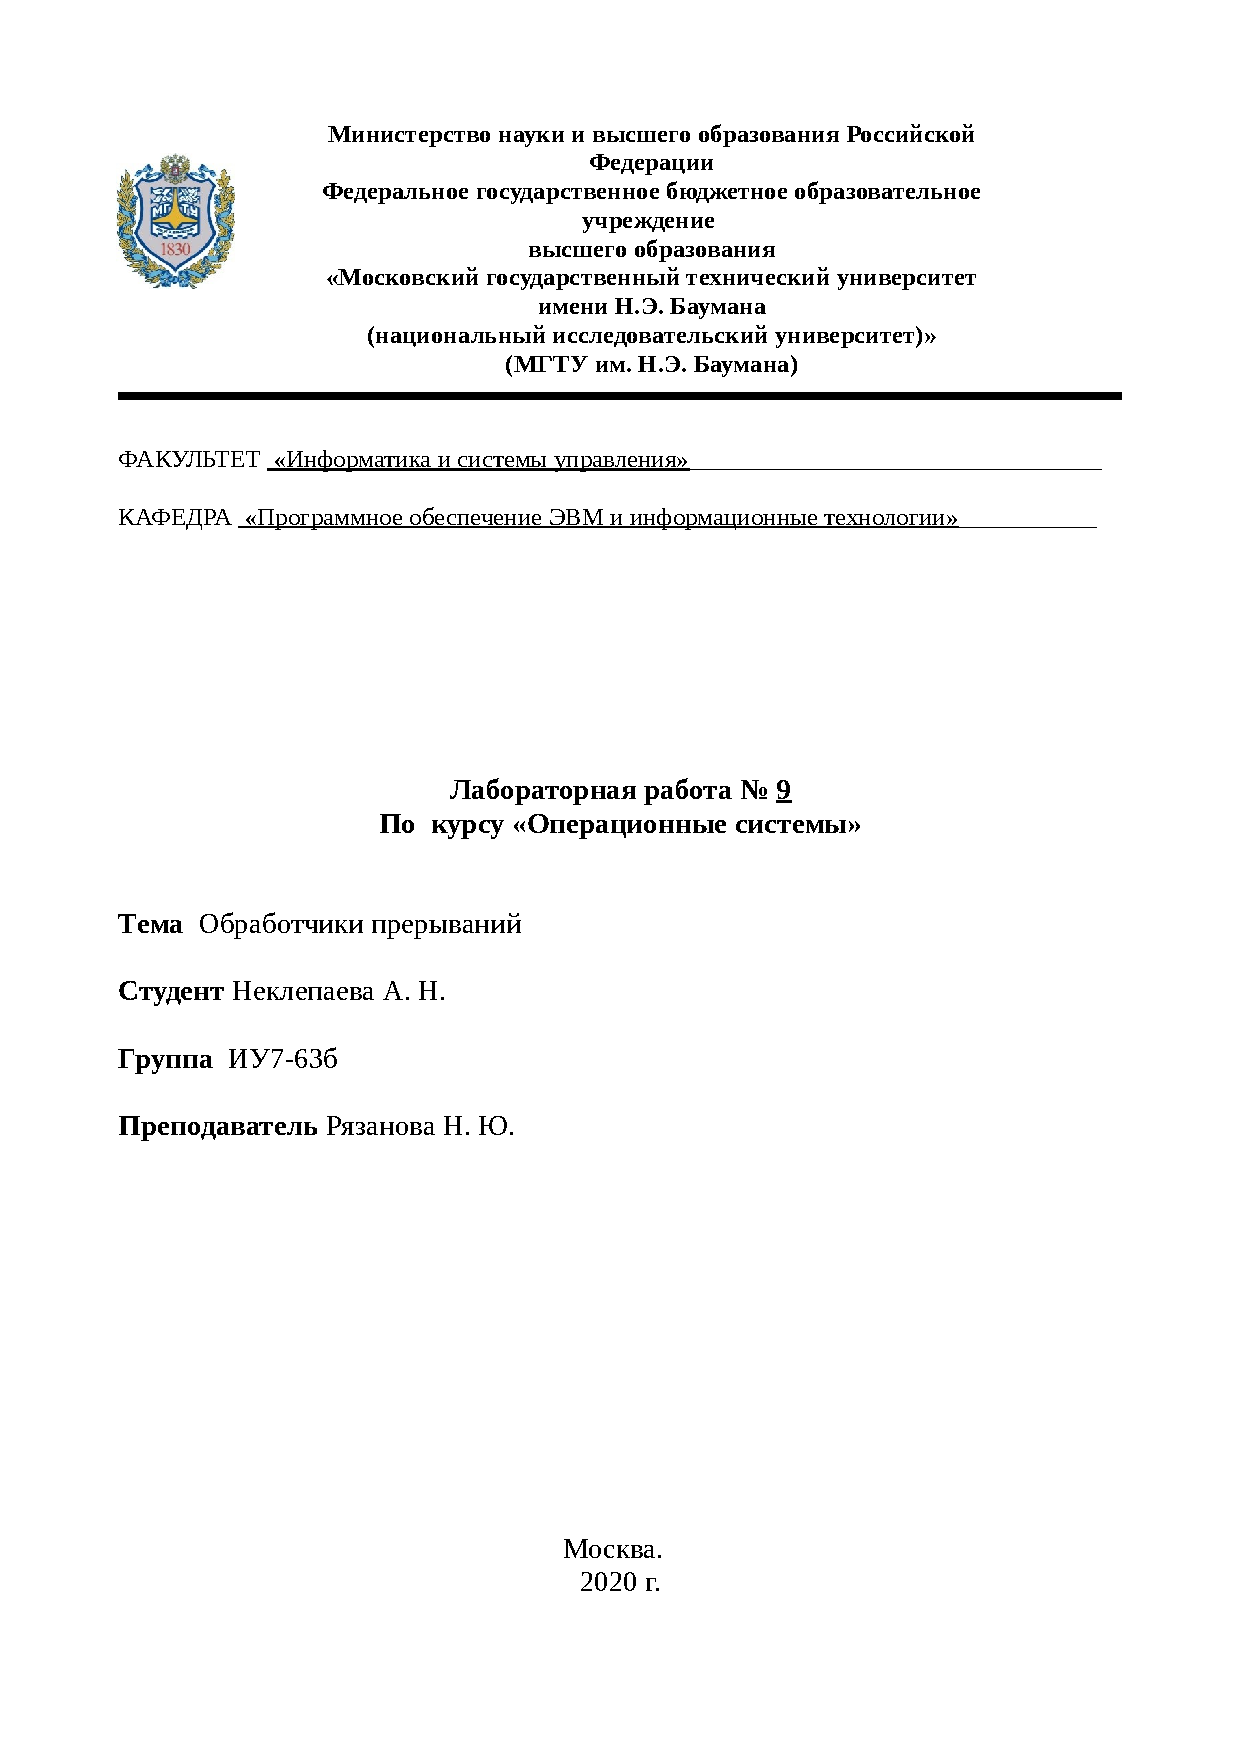
\includepdf[pages=-]{title.pdf}}
\end{figure}

\newpage

\textbf{Задание №1}\\
    • Написать загружаемый модуль ядра, в котором зарегистрировать обработчик аппаратного прерывания с флагом IRQF\underline{ }SHARED.\\
    • Инициализировать тасклет.\\
    • В обработчике прерывания запланировать тасклет на выполнение.\\
    • Вывести информацию о тасклете используя, или printk(), или seq\underline{ }file interface - <linux/seq\underline{ }file.h> (Jonathan Corber: http://lwn.net//Articales//driver-porting/).
    
\textbf{Листинг кода}

\begin{lstlisting}
  #include <linux/module.h>
  #include <linux/kernel.h>
  #include <linux/init.h>
  #include <linux/interrupt.h>
  #include <linux/sched.h>

  MODULE_LICENSE( "GPL" );
  MODULE_AUTHOR( "Anastasia Neklepaeva" );

  static int irq = 1;
  static int dev_id;
  void tasklet_func( unsigned long data );
  char tasklet_data[] = "tasklet_func was called";

  // keyboard controller
  #define DFN_IRQ 1

  // статическое создание тасклета
  DECLARE_TASKLET( tasklet, tasklet_func, (unsigned long) &tasklet_data );

  // обработчик прерывания
  static irqreturn_t irq_handler( int irq, void *dev_id ) 
  {
      if (irq == DFN_IRQ)
      {
          // запланирование тасклета на выполнение
          tasklet_schedule( &tasklet );
	  return IRQ_HANDLED; // прерывание обработано
      }
      else return IRQ_NONE; // прерывание не обработано
  }

  void tasklet_func(unsigned long data) 
  {
      // получение кода нажатой клавиши клавиатуры
      int code = inb(0x60);
      char * ascii[84] = 
      {" ", "Esc", "1", "2", "3", "4", "5", "6", "7", "8", "9", "0", "-", "+", "Backspace", 
       "Tab", "Q", "W", "E", "R", "T", "Y", "U", "I", "O", "P", "[", "]", "Enter", "Ctrl",
       "A", "S", "D", "F", "G", "H", "J", "K", "L", ";", "\"", "'", "Shift (left)", "|", 
       "Z", "X", "C", "V", "B", "N", "M", "<", ">", "?", "Shift (right)", 
       "*", "Alt", "Space", "CapsLock", 
       "F1", "F2", "F3", "F4", "F5", "F6", "F7", "F8", "F9", "F10",
       "NumLock", "ScrollLock", "Home", "Up", "Page-Up", "-", "Left",
       " ", "Right", "+", "End", "Down", "Page-Down", "Insert", "Delete"};
      if (code < 84) 
      {
          printk("+ tasklet: keyboard %s\n", ascii[code]);
      }
  }

  static int __init md_init( void )
  {
      // регистрация обработчика аппаратного прерывания
      int rc = request_irq(irq, irq_handler, IRQF_SHARED, "my_irq_handler", &dev_id);
      if (rc)
      {
          printk("+ tasklet: register interrupt handler error!\n" );
          return rc;
      }
      printk("+ tasklet: module loaded!\n" );
      return 0;
  }

  static void __exit md_exit( void )
  {
      tasklet_kill( &tasklet );
      free_irq( irq, &dev_id );
      printk("+ tasklet: module unloaded!\n" );
  }

  module_init( md_init );
  module_exit( md_exit );
\end{lstlisting}

\textbf{Демонстрация работы}

Загрузка модуля ядра\\
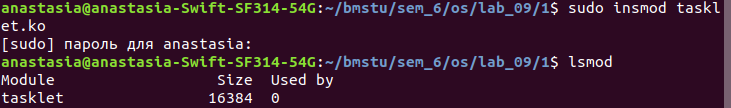
\includegraphics[scale=0.9]{1.png}

Выгрузка модуля, проверка системного лога\\
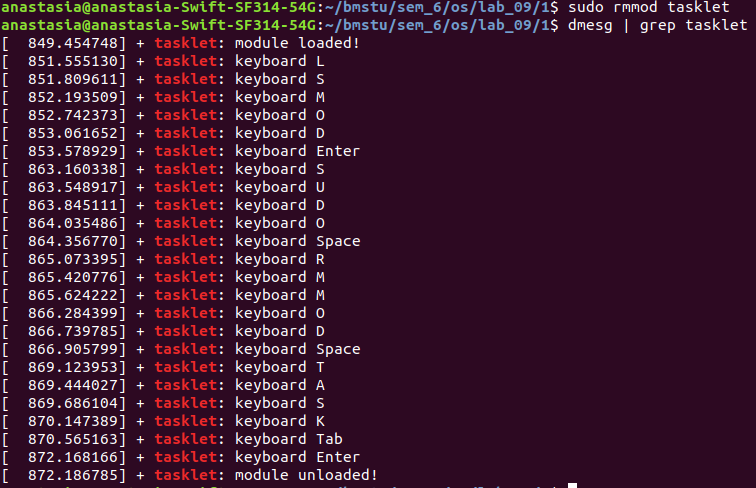
\includegraphics[scale=0.9]{2.png}

Вывод содержимого файла /proc/interrupts\\
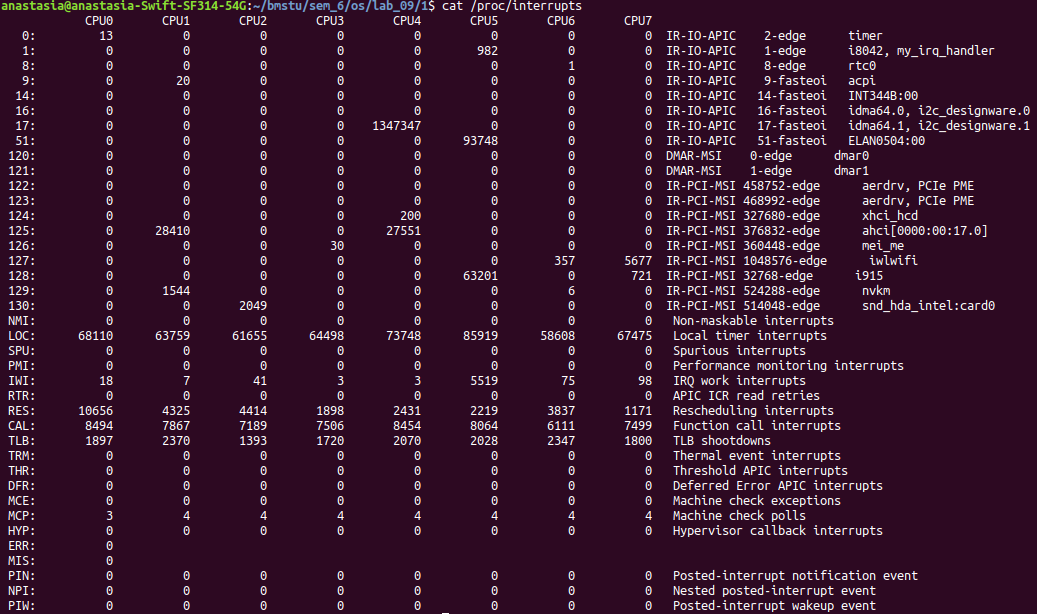
\includegraphics[scale=0.66]{3.png}

Видим разделение линии IRQ

\newpage

\textbf{Задание №2}\\
    • Написать загружаемый модуль ядра, в котором зарегистрировать обработчик аппаратного прерывания с флагом IRQF\underline{ }SHARED.\\
    • Инициализировать очередь работ.\\
    • В обработчике прерывания запланировать очередь работ на выполнение.\\
    • Вывести информацию об очереди работ используя, или printk(), или seq\underline{ }file interface - <linux/seq\underline{ }file.h> (Jonathan Corber: http://lwn.net//Articales//driver-porting/).
    
\textbf{Листинг кода}

\begin{lstlisting}
  #include <linux/module.h>
  #include <linux/kernel.h>
  #include <linux/init.h>
  #include <linux/interrupt.h>
  #include <linux/sched.h>
  #include <linux/workqueue.h>

  MODULE_LICENSE( "GPL" );
  MODULE_AUTHOR( "Anastasia Neklepaeva" );

  static int irq = 1;
  static int dev_id;
  struct workqueue_struct *workqueue;
  void work_func(struct work_struct *w);

  // keyboard controller
  #define DFN_IRQ 1

  // поместить задачу в очередь работ
  DECLARE_WORK(work, work_func);

  // обработчик прерывания
  static irqreturn_t irq_handler( int irq, void *dev_id ) 
  {
      if (irq == DFN_IRQ)
      {
          // добавление задачи в очередь работ
          queue_work(workqueue, &work);
	  return IRQ_HANDLED; // прерывание обработано
      }
      else return IRQ_NONE; // прерывание не обработано
  }

  void work_func(struct work_struct *w) 
  {
      // получение кода нажатой клавиши клавиатуры
      int code = inb(0x60);
      char * ascii[84] = 
      {" ", "Esc", "1", "2", "3", "4", "5", "6", "7", "8", "9", "0", "-", "+", "Backspace", 
       "Tab", "Q", "W", "E", "R", "T", "Y", "U", "I", "O", "P", "[", "]", "Enter", "Ctrl",
       "A", "S", "D", "F", "G", "H", "J", "K", "L", ";", "\"", "'", "Shift (left)", "|", 
       "Z", "X", "C", "V", "B", "N", "M", "<", ">", "?", "Shift (right)", 
       "*", "Alt", "Space", "CapsLock", 
       "F1", "F2", "F3", "F4", "F5", "F6", "F7", "F8", "F9", "F10",
       "NumLock", "ScrollLock", "Home", "Up", "Page-Up", "-", "Left",
       " ", "Right", "+", "End", "Down", "Page-Down", "Insert", "Delete"};
      if (code < 84) 
      {
          printk("+ workqueue: keyboard %s\n", ascii[code]);
      }
  }

  static int __init md_init( void )
  {
      // регистрация обработчика аппаратного прерывания
      int rc = request_irq(irq, irq_handler, IRQF_SHARED, "my_irq_handler", &dev_id);
      if (rc)
      {
          printk("+ workqueue: register interrupt handler error!\n" );
          return rc;
      }

      //создание очереди работ
      workqueue = create_workqueue( "workqueue" );

      if (!workqueue)
      {
          printk("+ workqueue: create_workqueue error!\n" );
          return -1;
      }

      printk("+ workqueue: module loaded!\n" );
      return 0;
  }

  static void __exit md_exit( void )
  {
      flush_workqueue(workqueue);
      destroy_workqueue(workqueue);
      free_irq( irq, &dev_id );
      printk("+ workqueue: module unloaded!\n" );
  }

  module_init( md_init );
  module_exit( md_exit );
\end{lstlisting}

\textbf{Демонстрация работы}

Загрузка модуля ядра\\
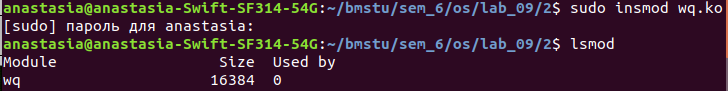
\includegraphics[scale=0.9]{4.png}

Выгрузка модуля, проверка системного лога\\
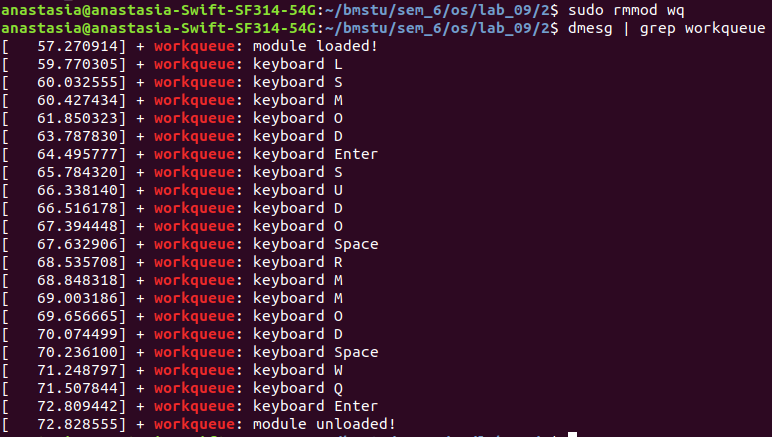
\includegraphics[scale=0.9]{5.png}

Вывод содержимого файла /proc/interrupts\\
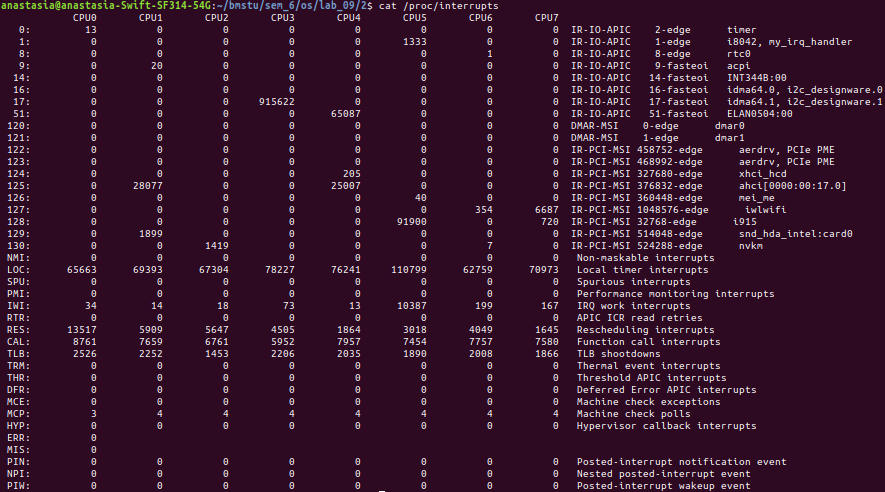
\includegraphics[scale=0.79]{6.png}

Видим разделение линии IRQ

\end{document}
